% *********************************************************************
% © 2010–2023 Jeremy Sylvestre
%
% Permission is granted to copy, distribute and/or modify this document
% under the terms of the GNU Free Documentation License, Version 1.3 or
% any later version published by the Free Software Foundation; with no
% Invariant Sections, no Front-Cover Texts, and no Back-Cover Texts. A
% copy of the license is included in the appendix entitled “GNU Free
% Documentation License” that appears in the output document of this
% PreTeXt source code. All trademarks™ are the registered® marks of
% their respective owners.
%
% *********************************************************************

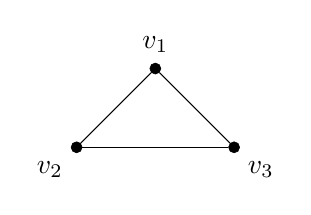
\begin{tikzpicture}[
	vertex/.style={ circle, draw, very thin, fill, inner sep=0pt, minimum size=4pt },
	vertexg/.style={ black!40!white, circle, draw, very thin, fill, inner sep=0pt, minimum size=4pt },
	vertexo/.style={ circle, draw, very thin, inner sep=0pt, minimum size=4pt }
]

\node at (1,1) (g1v1) [vertex,label=above:{$v_1$}] {};

\node at (0,0) (g1v2) [vertex,label=below left:{$v_2$}] {};
\draw (g1v2) to (g1v1);

\node at (2,0) (g1v3) [vertex,label=below right:{$v_3$}] {};
\foreach \p in {g1v1,g1v2} \draw (g1v3) to (\p);

\end{tikzpicture}
